% --- Άσκηση 38930 (38930.tex) ---
\Askhsh{38930}{4}
\begin{ylh}{2}
    \item 2.1. Οι Πράξεις και οι Ιδιότητές τους
    \item 6.2. Γραφική Παράσταση Συνάρτησης
\end{ylh}
\wrapr{-5mm}{12}{6.3cm}{-5mm}{
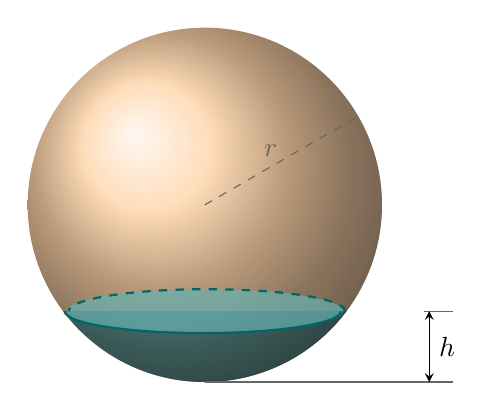
\begin{tikzpicture}[scale=1.5]
    \colorlet{spherespace}{orange!40!white}
    \colorlet{liquid}{teal!60!white}

    \def\R{1.5}
    \def\h{0.6}
    \def\y{-\R+\h}
    \pgfmathsetmacro\rliq{sqrt(\R*\R - \y*\y)}

    \shade[ball color=spherespace, opacity=0.9] (0,0) circle (\R);

    \begin{scope}
        \clip (-\R,-\R) rectangle (\R,\y);
        \shade[ball color=liquid, opacity=0.9] (0,0) circle (\R);
    \end{scope}

    \fill[liquid, opacity=0.7] (0,\y) circle[x radius=\rliq*0.63, y radius=\rliq*0.1];
    \draw[dashed, teal!80!black, thick,xshift=-0.67cm] (\rliq, \y) arc[start angle=0, end angle=180, x radius=\rliq*0.63, y radius=\rliq*0.1];
    \draw[teal!80!black, thick, xshift=0.67 cm] (-\rliq, \y) arc[start angle=180, end angle=360, x radius=\rliq*0.63, y radius=\rliq*0.1];

    \draw[dashed, thin, gray!80!black] (0,0) -- (30:\R) node[midway, above left=-2pt] {$r$};

    \draw[thin, gray!80!black] (\rliq, \y) -- (\R+0.6, \y);
    \draw[thin, gray!80!black] (0, -\R) -- (\R+0.6, -\R);
    \draw[<->, >=stealth] (\R+0.4, -\R) -- (\R+0.4, \y) node[midway, right] {$h$};
\end{tikzpicture}\captionof{figure}{Άσκηση 38930}}
{
Οι «κάψουλες με απορρυπαντικό» μπορούν να χρησιμοποιηθούν σε όλους τους τύπους πλυντηρίων ρούχων. Βοηθούν ώστε η πλύση να έχει καλύτερα αποτελέσματα (χωρίς χρήση μαλακτικού και πρόπλυσης).

\begin{alist}
\item Μια εταιρεία παράγει σφαιρικές κάψουλες ακτίνας $r = 2cm$ με το εξής χαρακτηριστικό: ο όγκος του σφαιρικού τμήματος ύψους$\ h$, που περιέχει το απορρυπαντικό, είναι ίσος με το 1/3 του όγκου της κάψουλας.

\begin{rlist}
\item Να δείξετε ότι το ύψος $h$ είναι λύση της εξίσωσης ${3h}^{3} - 18h^{2} + 32 = 0$.
\monades{8}
\item Στο παρακάτω σχήμα βλέπουμε τη γραφική παράσταση της συνάρτησης $f(x) = x^{3} - 6x^{2} + \dfrac{32}{3}$, για $- 1{,}5 < x < 6$.
Να αξιοποιήσετε την παραπάνω γραφική παράσταση, για να εκτιμήσετε το ύψος $h$ του σφαιρικού τμήματος που περιέχει το απορρυπαντικό, εξηγώντας τη σκέψη σας.
\monades{8}
\end{rlist}
\end{alist}}


\begin{center}
\begin{tikzpicture}
\begin{axis}[
    axis lines = middle,
    xlabel = {$x$},
    ylabel = {$y$},
    xmin = -2, xmax = 6.5,
    ymin = -25, ymax = 14,
    xtick = {-1,0,1,2,3,4,5,6},
    ytick = {-24,-20,...,12},
    grid = both,
    grid style = {gray!30},
    samples = 100,
    width = 11cm, height = 8cm,
    tick label style = {font=\small},
    every axis x label/.style = {at={(current axis.right of origin)}, anchor=north west},
    every axis y label/.style = {at={(current axis.above origin)}, anchor=south east},
]
